% Szablony LaTeX dla krzywych stabilności d(K) w funkcji parametru K w [3, 50]

\begin{figure}[htbp]
    \centering
    \begin{subfigure}[b]{0.48\textwidth}
        \centering
        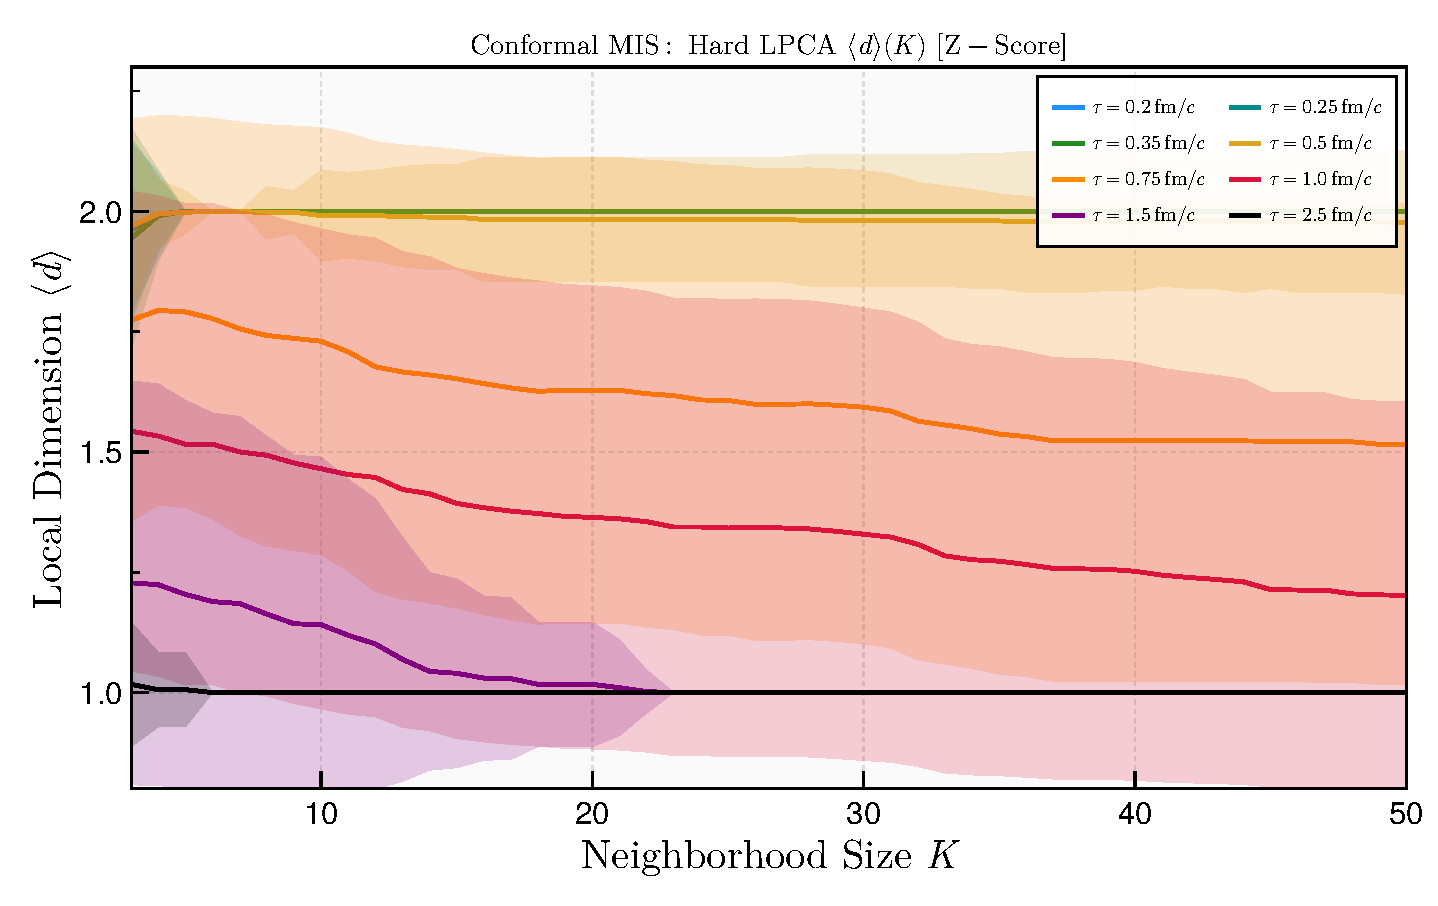
\includegraphics[width=\linewidth]{k_sweep_curves/k_sweep_mis_zscore_dims.pdf}
        \caption{MIS: \emph{dims} w funkcji $K$}
        \label{fig:k_sweep_mis_dims}
    \end{subfigure}
    \hfill
    \begin{subfigure}[b]{0.48\textwidth}
        \centering
        \includegraphics[width=\linewidth]{k_sweep_curves/k_sweep_mis_zscore_pr.pdf}
        \caption{MIS: \emph{pr} w funkcji $K$}
        \label{fig:k_sweep_mis_pr}
    \end{subfigure}

    \vspace{0.8em}

    \begin{subfigure}[b]{0.48\textwidth}
        \centering
        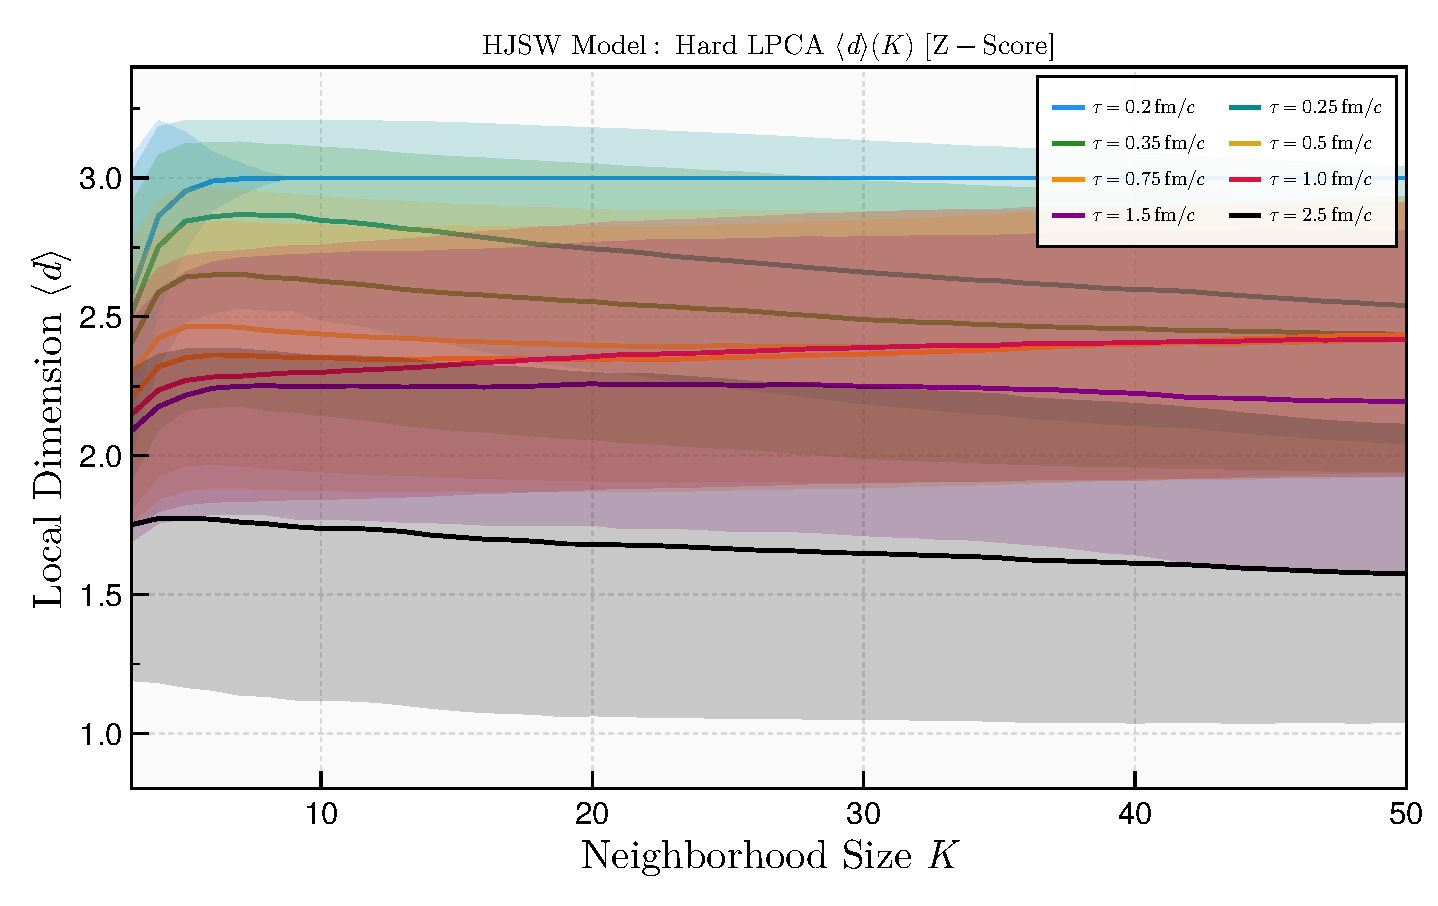
\includegraphics[width=\linewidth]{k_sweep_curves/k_sweep_hjsw_zscore_dims.pdf}
        \caption{HJSW: \emph{dims} w funkcji $K$}
        \label{fig:k_sweep_hjsw_dims}
    \end{subfigure}
    \hfill
    \begin{subfigure}[b]{0.48\textwidth}
        \centering
        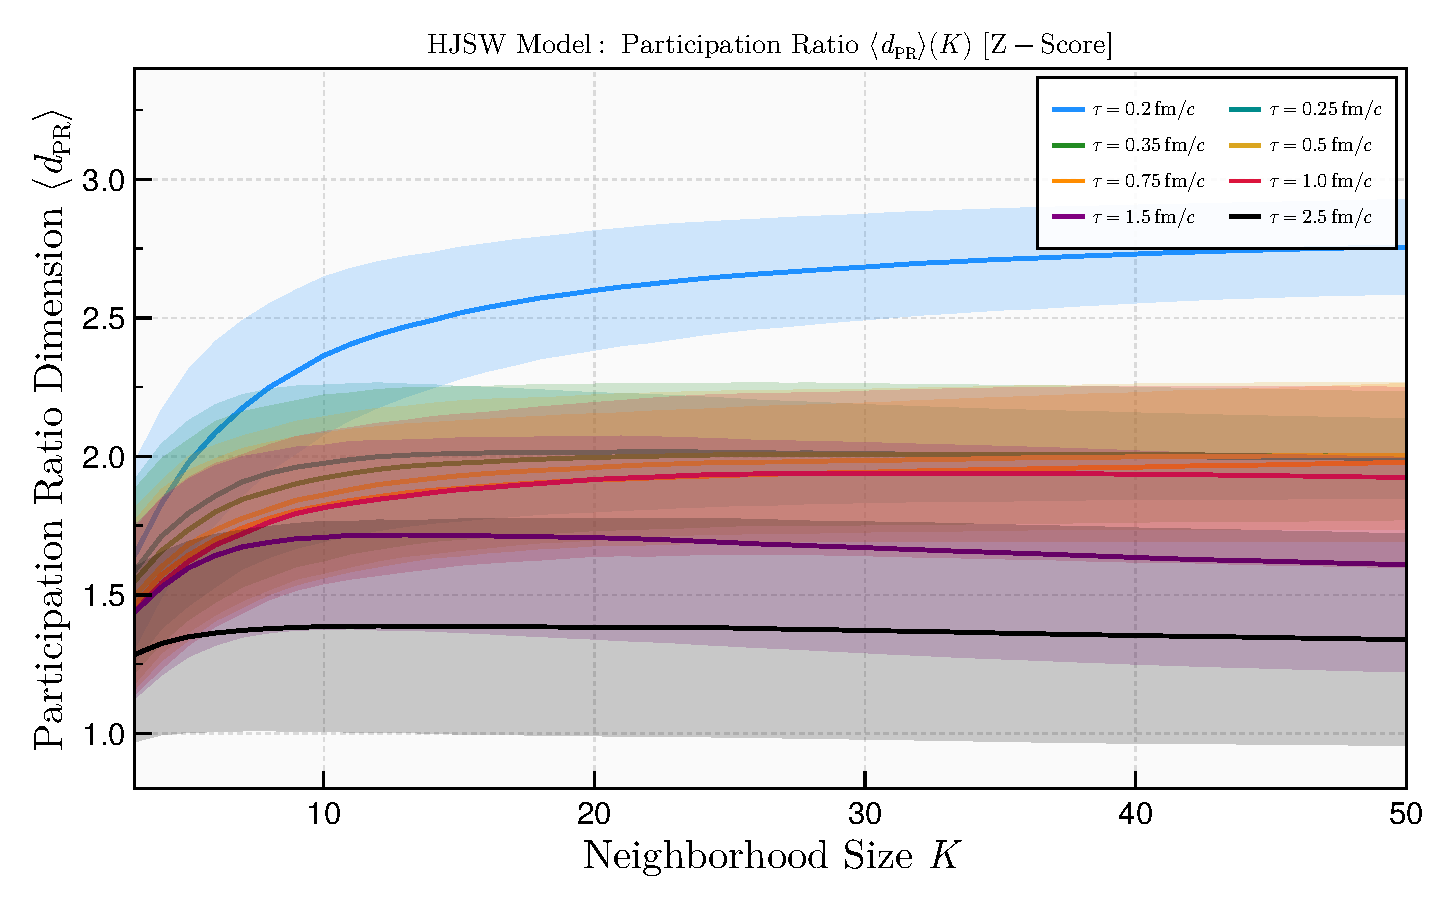
\includegraphics[width=\linewidth]{k_sweep_curves/k_sweep_hjsw_zscore_pr.pdf}
        \caption{HJSW: \emph{pr} w funkcji $K$}
        \label{fig:k_sweep_hjsw_pr}
    \end{subfigure}

    \caption{Zależność wyznaczonego wymiaru lokalnego od skali sąsiedztwa $K \in [3, 50]$ w standaryzacji Z-Score dla 8 wybranych przekrojów $\tau \in [0.20, 2.50]\,\mathrm{fm}/c$. Szeroki płaskowyż stabilności w przedziale $K \in [10, 40]$ potwierdza niezależność wyników od arbitralnego wyboru skali $k$-NN.}
    \label{fig:k_sweep_plateau}
\end{figure}
